\chapter{Die Spule}

%https://de.wikipedia.org/wiki/Datei:Electronic_component_inductors.jpg

\begin{wrapfigure}[0]{r}[-1cm]{3cm}
 \vspace{-5cm}
 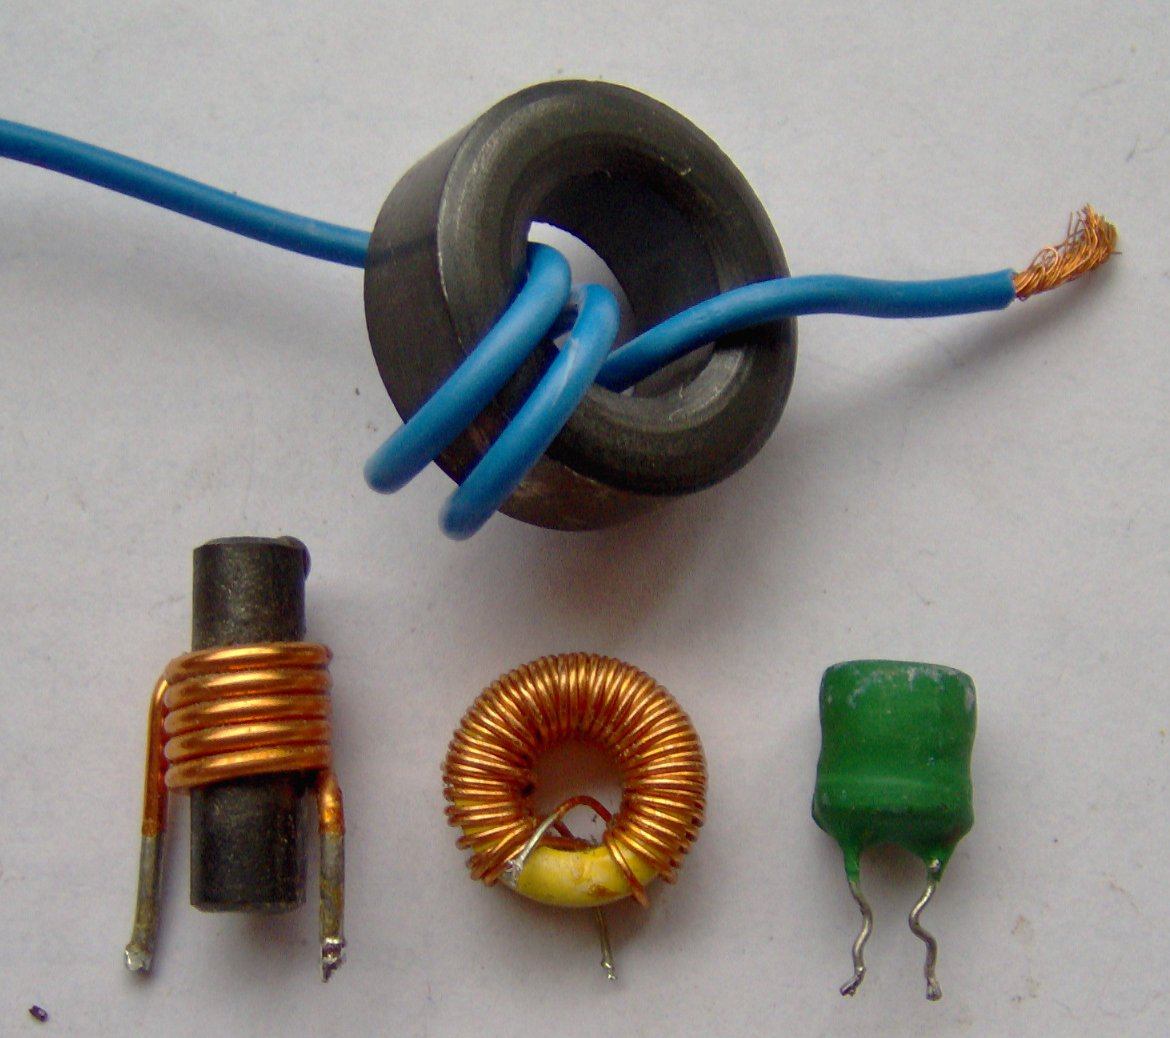
\includegraphics[scale=0.1]{Spule/Bilder/Electronic_component_inductors.jpg}
 \vspace{-5cm}
\end{wrapfigure}

\section*{Theorie- und Prüfungsfragen} 
~~~
\begin{enumerate}
\itemsep1pt\parskip0pt\parsep0pt
\item[1] Wie lässt sich die Induktivität einer Spule berechnen?
\item[2] Wie lautet die magnetische Feldkonstante $\mu_0$?
\item[3] Wie lautet die relative Permeabilität $\mu_r$ für Luft?
\item[4] Berechne die Induktivität der Zylinderspule mit folgender Bemaßung: 25 Windungen, 	Durchmesser von 8mm, Länge 1cm, relative Permeabilität von Luft
\end{enumerate}

\loesung{
	\begin{align}
	i) ~& L ~&=&~ & \dfrac{\mu_0 \cdot \mu_r \cdot A \cdot N^2}{l}\\
	ii) ~& \mu_0 ~&=&~ & 1,2566\cdot 10^{-6} \frac{H}{m}\\
	iii) ~& \mu_{r, Luft} ~& = &~ & 1 + 4 \cdot 10^{-7}\\
	iv) ~& L ~&=&~& 3,9\mu H
	\end{align}
	}

%\begin{block}
\aufgabentext{
	\begin{enumerate}
	\item[5] \emph{\textbf{TB402}}  Wie nennt man das Feld im Innern einer langen Zylinderspule beim Fließen eines Gleichstroms?
		\begin{enumerate}
		\itemsep1pt\parskip0pt\parsep0pt
		\item[A] Homogenes elektrisches Feld
		\item[B] Zentriertes magnetisches Feld
		\item[C] Konzentrisches Magnetfeld
		\item[D] Homogenes magnetisches Feld 
		\loesung{Lösung: D}
		\end{enumerate}
	\end{enumerate}
}

%\end{block}

%\begin{block}
\aufgabentext{
	\begin{enumerate}
	\item[6] \emph{\textbf{TC302}} Wie ändert sich die Induktivität einer Spule von $12 \mu H$, wenn die Wicklung auf dem Wickelkörper bei gleicher Windungszahl auf den doppelten Wert auseinander gezogen wird?
		\begin{enumerate}
		\itemsep1pt\parskip0pt\parsep0pt
			\item[A] Die Induktivität sinkt auf $3 \mu H$.
			\item[B] Die Induktivität sinkt auf $6 \mu H$. 
			\item[C] Die Induktivität steigt auf $24 \mu H$.
			\item[D] Die Induktivität steigt auf $48 \mu H$.
			\loesung{Lösung: B}
		\end{enumerate}	
	\end{enumerate}	
%\end{block}
}
%\begin{block}
\aufgabentext{
	\begin{enumerate}
		\item[7] \emph{\textbf{TC303}} Wie kann man die Induktivität einer Spule vergrößern?
		\begin{enumerate}
		\itemsep1pt\parskip0pt\parsep0pt
			\item[A] Durch Auseinanderziehen der Spule (Vergrößerung der Spulenlänge).
			\item[B] Durch Einführen eines Kupferkerns in die Spule.
			\item[C] Durch Stauchen der Spule (Verkürzen der Spulenlänge). 
			\item[D] Durch Einbau der Spule in einen Abschirmbecher.
			\loesung{Lösung: C}
		\end{enumerate}
	\end{enumerate}
%\end{block}
}



\mucho{8}{TC305}
{Schaltet man zwei Glühlampen gleichzeitig an eine Spannungsquelle (siehe Abbildung), wobei eine Glühlampe zum Helligkeitsausgleich über einen Widerstand und die andere über eine Spule mit vielen Windungen und Eisenkern angeschlossen ist, so\\ 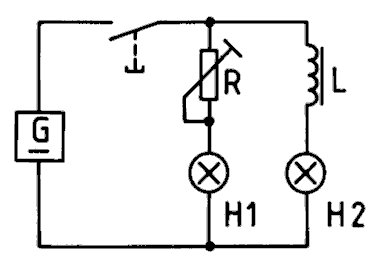
\includegraphics[scale=0.35]{Spule/Bilder/TC305.png}}%Frage
{leuchtet H1 zuerst.}%A
{leuchtet H2 zuerst.}%B
{leuchten H1 und H2 genau gleich schnell.}%C
{leuchtet H2 kurz auf und geht wieder aus. H1 leuchtet.}%D
{A}%Lösung

\mucho{9}{TC402}
{Ein Trafo liegt an 45 Volt und gibt 180 Volt ab. Seine Primärwicklung hat 150 Windungen. Wie groß ist seine Sekundärwindungszahl?}%Frage
{46 Windungen}%A
{30 Windungen}%B
{600 Windungen}%C
{850 Windungen}%D
{C: $\dfrac{N_1}{N_2} = \dfrac{U_1}{U_2}$; $N_2 = \dfrac{180V}{45V} \cdot 150$}%Lösung

\mucho{10}{TC403}
{Die Primärspule eines Übertragers hat die fünffache Anzahl von Windungen der Sekundärspule. Wie hoch ist die erwartete Sekundärspannung, wenn die Primärspule an eine 230-V-Stromversorgung angeschlossen wird?}%Frage
{46 Volt}%A
{9,2 Volt}%B
{23 Volt}%C
{1150 Volt}%D
{A: $\dfrac{N_1}{N_2} = \dfrac{U_1}{U_2}$; $U_2 = \dfrac{1}{5} \cdot 230V$}%Lösung

\mucho{11}{TC304}
{Das folgende Bild zeigt einen Kern, um den ein Kabel für den Bau einer Netzdrossel gewickelt ist. Der Kern sollte aus\\ 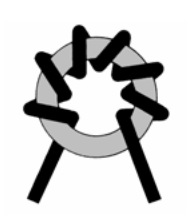
\includegraphics[scale=0.9]{Spule/Bilder/TC304.png}}%Frage
{Kunststoff bestehen.}%A
{Ferrit bestehen.}%B
{Stahl bestehen.}%C
{aus gut leitendem Material bestehen.}%D
{B}%Lösung

\mucho{12}{TC306}
{Mit zunehmender Frequenz}%Frage
{sinkt der Wechselstromwiderstand einer Spule.}%A
{sinkt der Wechselstromwiderstand einer Spule
bis zu einem Minimum und steigt dann wieder.}%B
{steigt der Wechselstromwiderstand einer Spule
bis zu einem Maximum und sinkt dann wieder.}%C
{steigt der Wechselstromwiderstand einer Spule.}%D
{D}%Lösung

%----------------------------
\newpage

\section*{Praktische Anwendung}

\subsection*{Spule wickeln}

% FIXME Foto einer eigenen Spule
\begin{wrapfigure}{r}{0.4\textwidth}
 \vspace{-10pt}
 \centering 
 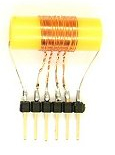
\includegraphics[scale=4]{Spule/Bilder/Spule_bau.jpg}
 %\caption{Bildunterschrift der Grafik.}
 %\label{fig:meine-Grafik}
 \vspace{-5pt}
\end{wrapfigure}

% Sollte auf Mehrband-RX hinführen - ist aber zu aufändig
% Für den ersten Versuch soll eine Spule mit insgesamt $25 $Windungen und vier
% Anzapfungen gewickelt werden. Als Wickelkörper soll eine 8 mm dickes und $3cm$
% langes Stück eines Trinkhalmes verwendet werden. Zwei Löcher im Abstand $1cm$
% helfen die Drahtenden zu fixieren. Es werden dann jeweils $5$ Windungen
% gewickelt, eine Schlaufe verdrillt und die folgenden Windungen aufgetragen. Die
% fertige Spule wird an einen Abschnitt Pfostenstecker mit sechs Kontakten
% gelötet. 

Für den ersten Versuch soll eine Spule aus $1 m$ Kupferlackdraht gewickelt
werden. Denkt daran beim Wickeln die Windungszahl zu zählen!

\begin{enumerate}
  \item Als Wickelkörper dient ein $8 mm$ dickes und $3cm$ langes Stück eines
    Trinkhalmes.
  \item Zwei Löcher im Abstand $1cm$ helfen die Drahtenden zu fixieren.
  \item Um die Kontakte der Spule frei zu legen, muss die aufgetragene
    Lackschicht abgeschabt oder mit einem Feuerzeug freigebrannt werden.
  \item Berechnet die Induktivität $L$ eurer Spule und messt mit dem
    LC-Messgerät nach.
\end{enumerate}

\loesung{Die Spule sollte um die $3-5 uH$ haben, damit der darauf aufbauende
KW-Empfänger-Versuch mit einem Schwingkreis um die $7 MHz$ klappt.}

\subsection*{Impedanz von C und L}

Wdh. Kondensator:

\begin{itemize}
    \item Erzeuge mit den Klinkenanschlusskabel und einem Signalgenerator
      Sinusschwingungen und finde heraus in welchem Bereich die Schwingungen
      noch deutlich hörbar sind.
    \item Schleife nun einen Koppelkondensator mit $C = 100 nF$ ein. Welche Unterschiede
      sind hörbar? \loesung{Hochpassverhalten}
    \item Berechne die Impedanz der Kondensators in den oberen und unteren
      Bereichen der Hörschwelle.
    \item Zusatzaufgabe: Was passiert mit einem Rechtecksignal?
\end{itemize}

% TODO Induktivität/Kapazität als Energiespeicher:
%      * siehe Experiment TC305
%      * Glimmlampen
%      * mit Dioden antiparallel?

Spule:

\begin{itemize}
  \item Wiederholt das o.g. Experiment mit eurer Spule -- was fällt euch auf?
  \item Wiederholt das o.g. Experiment noch einmal mit einer geg. Spule -- hier
    reicht das Messen der Impedanz % FIXME
\end{itemize}

\loesung{Ziel in diesem Teil ist es herauszufinden, dass es unglaubliche
Windugszahlen bei Spulen erfordert um etwas im niederfrequenten Bereich zu
erreichen.}

% DONE Spannungsteilerversuch mit 1 Ohm und Induktivität von bis zu 20 uH
%      fehlgeschlagen :-( Allein die Übergangswiderstände machen schon zu viel aus
% TODO einfaches Audiofilter als Notch?
% TODO Induktionsversuch a la Trafo?

